\chapter{Fundamentals}
\label{ch:fundamentals}
	Understanding this paper requires knowledge about certain terms. These terms are defined and illustrated in this chapter.

	\section{Text Classification}
	\label{sec:classification}
		Text classification is a special topic within the more general field of text mining which tries to extract useful information from unstructured texts.\autocite{Baharudin.2010} Text classification does this by labeling a text with its corresponding class labels. A text can correspond to only one class (single-label) or more classes (multi-label). Assigning only one label out of several classes is called multi-class classification while assigning several labels is called multi-label classification.
		\par
		It is common to represent the class distribution of a text with a one-hot array for multi-class classification or a multi-hot array for multi-label classification. Each scalar of the vector represents the probability of a given class. For example, imagine classifying recruitment advertisements for baker, barber and butcher. In this example the class distribution vector has three scalars the first one corresponding to baker, the second one to barber and the third one to butcher. In consequence, a golden vector for a bakers recruitment advertisement looks like \eqref{eq:1hot}.
		\begin{equation}
			\label{eq:1hot}
			\begin{pmatrix}
				1\\
				0\\
				0\\
			\end{pmatrix}
		\end{equation}
		For neural multi-class classification this is achieved using the softmax activation function. The softmax function represents a probability distribution over all classes. Therefore, the golden vector has the probability $1$ for the recruitment advertisements class and $0$ for all other classes. As the predicted vector is most likely not equal to the golden vector, the class with the highest scalar value is taken as the predicted class.\autocite{Krause.2017}
		For multi-label classification this does not work, as the golden vector can contain several probabilities of $1$. Because of this the sigmoid or logistics activation function is used. The sigmoid activation function \enquote{squashes} all values into the range $[0;1]$. \autocite{Krause.2017} Here again, the predicted vector is most likely not equal to the golden vector. That is why a threshold is used to decide whether a classes is taken as predicted or not. All classes with a corresponding scalar value above a certain threshold are taken as predicted. \autocite{LeCun.2015}

	\section{Neuron}
		\label{sec:neuron}
		A neuron is the basic unit of a neural network. A neuron consists of  $n$ weighted connections  $w_i, i \in [1;n]$, a sum function $\sum$ and an activation function $\varphi$\autocite{Jain.1996}, see Figure \ref{img:neuron}. Common activation functions are sigmoid, tanh and \ac{ReLU}. In recent years \ac{ReLU} is commonly used.\autocite{LeCun.2015} Chaining these operations produces the output $y$ of a neuron. Given an input $\vec{x}$ this operator chain results in Equation \eqref{eq:neuron:y}.\autocite{Jain.1996}
		\begin{equation}
			\label{eq:neuron:y}
			\begin{array}{lcl}
			y & = & \varphi(\sum_{i=1}^{n} x_i \cdot w_i)\\
			& = & \varphi(\vec{w}^{\mathrm {T}} \cdot \vec{x}) | \vec{w}^{\mathrm {T}}=(w_1, w_2 \dots w_n)
			\end{array}
			\end{equation}
		\begin{figure}[H]
			\centering
			\begin{tikzpicture}
			\node (x0) at (0,3) {$x_0$};
			\node (x1) at (0,2) {$x_1$};
			\node (..) at (0,1) {$\vdots$};
			\node (xn) at (0,0) {$x_n$};
			\node[draw, circle, minimum size=1cm] (sum) at (2,1.5) {$\sum$};
			\node[draw, circle, minimum size=1cm] (phi) at (4,1.5) {$\varphi$};
			\node (y) at (6,1.5) {$y$};
			\draw[->] (x0) -- (sum) node[sloped,pos=.3,above] {$w_0$};
			\draw[->] (x1) -- (sum) node[sloped,pos=.3,above] {$w_1$};
			\draw[->] (xn) -- (sum) node[sloped,pos=.3,above] {$w_n$};
			\draw[->] (sum) -- (phi);
			\draw[->] (phi) -- (y);
			\node[draw,	ellipse, minimum height=2cm,minimum width=3cm, label=Neuron] (neuron) at (3,1.5) {};
			\end{tikzpicture}
			\caption{Neuron (own figure)} \label{img:neuron}
		\end{figure}

	\section{\ac{MLP}}
	\label{sec:mlp}
		A \ac{MLP} or multilayer feed forward network is a basic neural network structure. A \ac{MLP} consists of interconnected neurons. The neurons are arranged in $m$ layers $l \in [0,m]$. A layer can contain any number $n$ of neurons. Each neuron of layer $l$ is connected to each neuron in layer $l-1$, see Figure \ref{img:nnexample}. \autocite{Svozil.1997} The connections between two layers can be described in a matrix. Given the neurons $n_{kl}$ in row $k, k \in [0,n]$ of layer $l$, the weight $w_{ij}$ describes the connection between the neuron $n_{jl-1}$ in row $j$ of the previous layer $l-1$ and the neurons $n_{il}$ in row $i$ of the layer $l$. In consequence, each layer possesses an own weight matrix $W_l$. In this matrix the weights describing all incoming connections of a neuron $n_{kl}$ are arranged in row $k$. This row corresponds to the transposed weight vector of a neuron $\vec{w}^{\mathrm {T}}$, as described in Equation \eqref{eq:neuron:y}. Resulting therefrom, applying an element wise activation function to the product of the weight matrix $W_l$ and the input vector $\vec{x_l}$ of a layer results in the output vector of that layer $\vec{y_l}$. This operation chain is described by Equation \ref{eq:nn:y}. Consequently, this equation can be seen as applying a linear vector space transformation followed by a non linear vector space transformation of the layers input.
		\begin{equation}
			\label{eq:nn:y}
			\vec{y_l} = \varphi(W_l \cdot \vec{x_l})
		\end{equation}
		\begin{figure}[H]
			\centering
			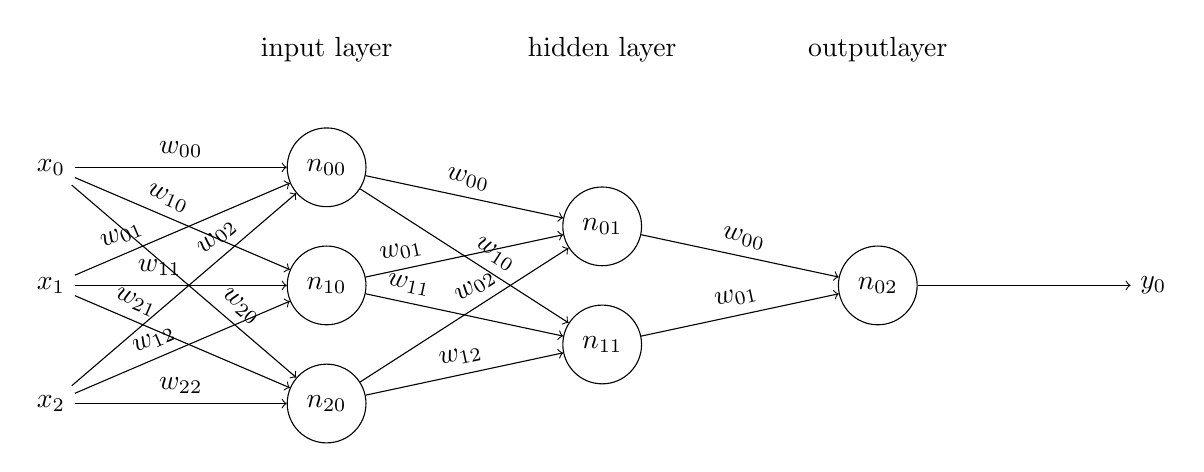
\begin{tikzpicture}
				% input
				\node (x0) at (0,3) {$x_0$};
				\node (x1) at (0,1.5) {$x_1$};
				\node (x2) at (0,0) {$x_2$};
				% input layer
				\node[align=center, text width=20em] (ins) at (3.5,4.5) {input layer};
				\node[draw, circle, minimum size=1cm] (n00) at (3.5,3) {$n_{00}$};
				\node[draw, circle, minimum size=1cm] (n10) at (3.5,1.5) {$n_{10}$};
				\node[draw, circle, minimum size=1cm] (n20) at (3.5,0) {$n_{20}$};
				% hidden layer
				\node[align=center, text width=20em] (hs) at (7,4.5) {hidden layer};
				\node[draw, circle, minimum size=1cm] (n01) at (7,2.25) {$n_{01}$};
				\node[draw, circle, minimum size=1cm] (n11) at (7,0.75) {$n_{11}$};
				% output layer
				\node[align=center, text width=20em] (hs) at (10.5,4.5) {outputlayer};
				\node[draw, circle, minimum size=1cm] (n02) at (10.5,1.5) {$n_{02}$};
				% output
				\node (y) at (14,1.5) {$y_0$};
				% input -> input layer
				\draw[->] (x0) -- (n00) node[sloped,pos=.50,above] {$w_{00}$};
				\draw[->] (x0) -- (n10) node[sloped,pos=.40,above] {$w_{10}$};
				\draw[->] (x0) -- (n20) node[sloped,pos=.70,above] {$w_{20}$};
				\draw[->] (x1) -- (n00) node[sloped,pos=.25,above] {$w_{01}$};
				\draw[->] (x1) -- (n10) node[sloped,pos=.40,above] {$w_{11}$};
				\draw[->] (x1) -- (n20) node[sloped,pos=.25,above] {$w_{21}$};
				\draw[->] (x2) -- (n00) node[sloped,pos=.70,above] {$w_{02}$};
				\draw[->] (x2) -- (n10) node[sloped,pos=.40,above] {$w_{12}$};
				\draw[->] (x2) -- (n20) node[sloped,pos=.50,above] {$w_{22}$};
				% input layer -> hidden layer
				\draw[->] (n00) -- (n01) node[sloped,pos=.5,above] {$w_{00}$};
				\draw[->] (n00) -- (n11) node[sloped,pos=.6,above] {$w_{10}$};
				\draw[->] (n10) -- (n01) node[sloped,pos=.2,above] {$w_{01}$};
				\draw[->] (n10) -- (n11) node[sloped,pos=.2,above] {$w_{11}$};
				\draw[->] (n20) -- (n01) node[sloped,pos=.6,above] {$w_{02}$};
				\draw[->] (n20) -- (n11) node[sloped,pos=.5,above] {$w_{12}$};
				% hidden layer -> output layer
				\draw[->] (n01) -- (n02) node[sloped,pos=.5,above] {$w_{00}$};
				\draw[->] (n11) -- (n02) node[sloped,pos=.5,above] {$w_{01}$};
				% output layer -> output
				\draw[->] (n02) -- (y);
			\end{tikzpicture}
			\caption{\ac{MLP} Illustration (own figure)} \label{img:nnexample}
		\end{figure}
		\par
		Figure \ref{fig:nn_matrix} illustrate the transfer of the connections between two layers to their matrix representation. In this illustration all incoming connections of a neuron are highlighted in the same color. These connections are described by the transposed weight vector of that neuron. The transposed weight vectors are highlighted in the same color as their corresponding connections. Concatenating these transposed weight vectors results in the weight matrix of that layer. For reasons of simplicity, in this illustration the activation function $\varphi_0$ is the identity function.
		\begin{figure}[H]
			\centering
			\begin{tikzpicture}
	\node (x0) at (0,1.5) {$8$};
	\node (x1) at (0,0) {$9$};
	\node[draw, circle, minimum size=1cm] (n00) at (2,1.5) {$n_{00}$};
	\node[draw, circle, minimum size=1cm] (n10) at (2,0) {$n_{10}$};
	\node (y0) at (4,1.5) {$35$};
	\node (y1) at (4,0) {$52$};
	\draw[->, blue] (x0) -- (n00) node[sloped,pos=.50,above] {$1$};
	\draw[->, orange] (x0) -- (n10) node[sloped,pos=.40,above] {$2$};
	\draw[->, blue] (x1) -- (n00) node[sloped,pos=.40,above] {$3$};
	\draw[->, orange] (x1) -- (n10) node[sloped,pos=.50,above] {$4$};
	\draw[->] (n00) -- (y0);
	\draw[->] (n10) -- (y1);
	\node (equation) at (2,-2) {$
		\vec{y_0} = \varphi_0(M_0 \cdot \vec{x_0}) =
		\varphi_0 \left( 
		\begin{pmatrix}
			\textcolor{blue}{1} & \textcolor{blue}{3}\\
			\textcolor{orange}{2} & \textcolor{orange}{4}
		\end{pmatrix} \cdot
		\begin{pmatrix}
			8\\
			9
		\end{pmatrix} \right)
		= \varphi_0\left(
		\begin{pmatrix}
			\textcolor{blue}{1} \cdot 8 + \textcolor{blue}{3} \cdot 9\\
			\textcolor{orange}{2} \cdot 8 + \textcolor{orange}{4} \cdot 9
		\end{pmatrix} \right)
		= 
		\begin{pmatrix}
			35\\
			52
		\end{pmatrix}
		$};
\end{tikzpicture}
			\caption{Illustration of the Matrix Representation (own figure)} \label{fig:nn_matrix}
		\end{figure}
		\par
		Additionally to neurons a layer may contain bias units. A bias unit is a neuron without any input and an output of $1$. Therefore, a bias just adds its weights to the neurons it is connected to. Consequently the impact of a bias on a layer can be described by a bias weight vector $b_l$, see Equation \eqref{eq:bias}.
		\begin{equation}
			\label{eq:bias}
			\vec{y_l} = \varphi(W_l \cdot \vec{x_l} + b_l)
		\end{equation}
		A \ac{MLP} consists of several layers. The first layer is called the input layer, the last layer is called the output layer and any other layer is called hidden layer. Each layer uses the output of the previous layer as its own input, except for the input layer, which receives the networks input $\vec{x}$ .\autocite{Svozil.1997} As a result, the \ac{MLP} can be described as a chain of layers resulting in Equation \eqref{eq:nn}.
		\begin{equation}
			\label{eq:nn}
			\vec{y} = \varphi(W_m \cdot \dots\varphi(W_1 \cdot \varphi(W_0 \cdot \vec{x} + b_0) + b_1)\dots + b_m)
		\end{equation}
			
	\section{Learning with Neural Networks}
		Machine learning in general is the art of training an algorithm to generate new information from data. The goal of machine learning is not to model explicitly how to extract this information, but to let the computer itself learn the model. \autocite{Mohri.2012}
		\par
		A neural network is an universal function approximator.\autocite{Hornik.1989} Meaning, they can learn any function, for example classifying recruitment advertisements as barber, baker and butcher. How well a neural network approximates a function is measured by an objective function $\mathcal{L}$. The objective function usually represents some kind of error on a given task. Hence, it is the goal to minimize that function. This is done by adjusting the neural network's parameters $\theta$. To properly adjust $\theta$, backpropagation \autocite{Rumelhart.1986} is used to calculate a gradient vector $\partial \theta$. This gradient indicates by what amount the error increases or decreases if $\theta$ is increased by a tiny amount. The objective function with regard to $\theta$ can be seen as high-dimensional hilly landscape, with the negative gradient vector indicating the direction of steepest descent in that landscape. This gradient is used to descend in that landscape to find the minimum. In practice, usually stochastic gradient descent is used to minimize the objective function. \autocite{LeCun.2015}
		\paragraph{Supervised Learning}
		is learning using an objective function that measures the error (or distance) between the actual output of the neural network and the desired output. Therefore, a large dataset of labeled input data is required. In regard to the given example, this dataset consists of recruitment advertisements labeled by their corresponding class. After training the performance of the system is measured on a different set of examples called a test set. This serves to test the generalization ability of the machine. The generalization ability is the ability to produce sensible outputs on new inputs not seen during training. \autocite{LeCun.2015}
		\paragraph{Unsupervised Learning}
		is learning without knowing the desired output. \autocite{Ghahramani.2004} In regard to the given example, in the case of unsupervised learning the classes corresponding to the recruitment advertisements are unknown.
		
	\section{Transfer Learning and Pre-Training}
	\label{sec:learning}
	Transfer learning aims to help learning a specific task by learning another task. For example, learning the classification of recruitment advertisements requires some form of learning a language. This applies to the task of language modeling as well. Consequently, training a model for language modeling might help to learn the classification of recruitment advertisements. 
	\par
	Transfer learning is defined as follows: \blockcquote{Pan.2010}{Given a source domain $\mathcal{D_S}$ and  learning  task $\mathcal{T_S}$,  a  target  domain $\mathcal{D_T}$ and  learning  task $\mathcal{T_T}$, transfer learning aims to help improve the learning of the target predictive function $f_{\mathcal{T}}(\cdot)$ in $\mathcal{D_T}$ using the knowledge in $\mathcal{D_S}$ and $\mathcal{T_S}$, where $\mathcal{D_S}\ne\mathcal{D_T}\text{, or } \mathcal{T_S} \ne \mathcal{T_T}$}. 
	A domain $\mathcal{D}=\{\mathcal{X},P(X)\}$ is comprised of a feature space $\mathcal{X}$ and a probability distribution $P(X) \text{, } X=\{x_1,x_2,\dots,x_n\} \in \mathcal{X}$. A feature space is a vector space containing a vector embedding for each input. In regard to the given example, the recruitment advertisement are a corpus of words. These words can be embedded via vectors, which form a sequence of vectors. This sequence of vectors is the input to the classifier. Resulting from that, the vector space in which the input is located is called feature space.
	A task  $\mathcal{T}=\{\mathcal{Y},f(\cdot)\}$ is comprised of a label space $\mathcal{Y}$ and a prediction function $f(\cdot)$. In the given example, recruitment advertisements are labeled by their job titles. These titles are the classes of this classification task. As explained in Section \ref{sec:classification}, for this example, each class distribution can be represented with a one-hot vector. Hence, the vector space containing these one-hot vectors is called label space. For this task, the objective of the prediction function $f(\cdot)$ is to predict the corresponding class $f(x_i)=y_i \in \mathcal{Y}$ from an input $x_i \in \mathcal{X}$. That means to predict the job title corresponding to a recruitment advertisement. \autocite{Pan.2010}
	\par
	Pre-training and fine-tuning is a form of transfer learning. Pre-training refers to training a model on a source task solely for the purpose of learning the target task faster. For pre-training, the model is trained on a source task with a vast amount of training data available. Usually, an unsupervised task, like a kind of language modeling, is used. Subsequently, the model is fine-tuned. For fine-tuning, the model is initialized with the parameters learned in the pre-training and trained on the target task. \autocites{Joshi.2019}{Devlin.2018}{Liu.2019}{Radford.2018}{Yang.2019}{Howard.2018}
	This is especially useful for target tasks with few training data.